% !TeX root = ../../../main.tex
\begin{figure}[htbp]
\begin{ChFiveFloatBody}

    \centering
    \subfloat[{Most frequent diagnoses.}]{\begin{minipage}[t]{0.39\textwidth}
        \centering
        \raisebox{40pt}{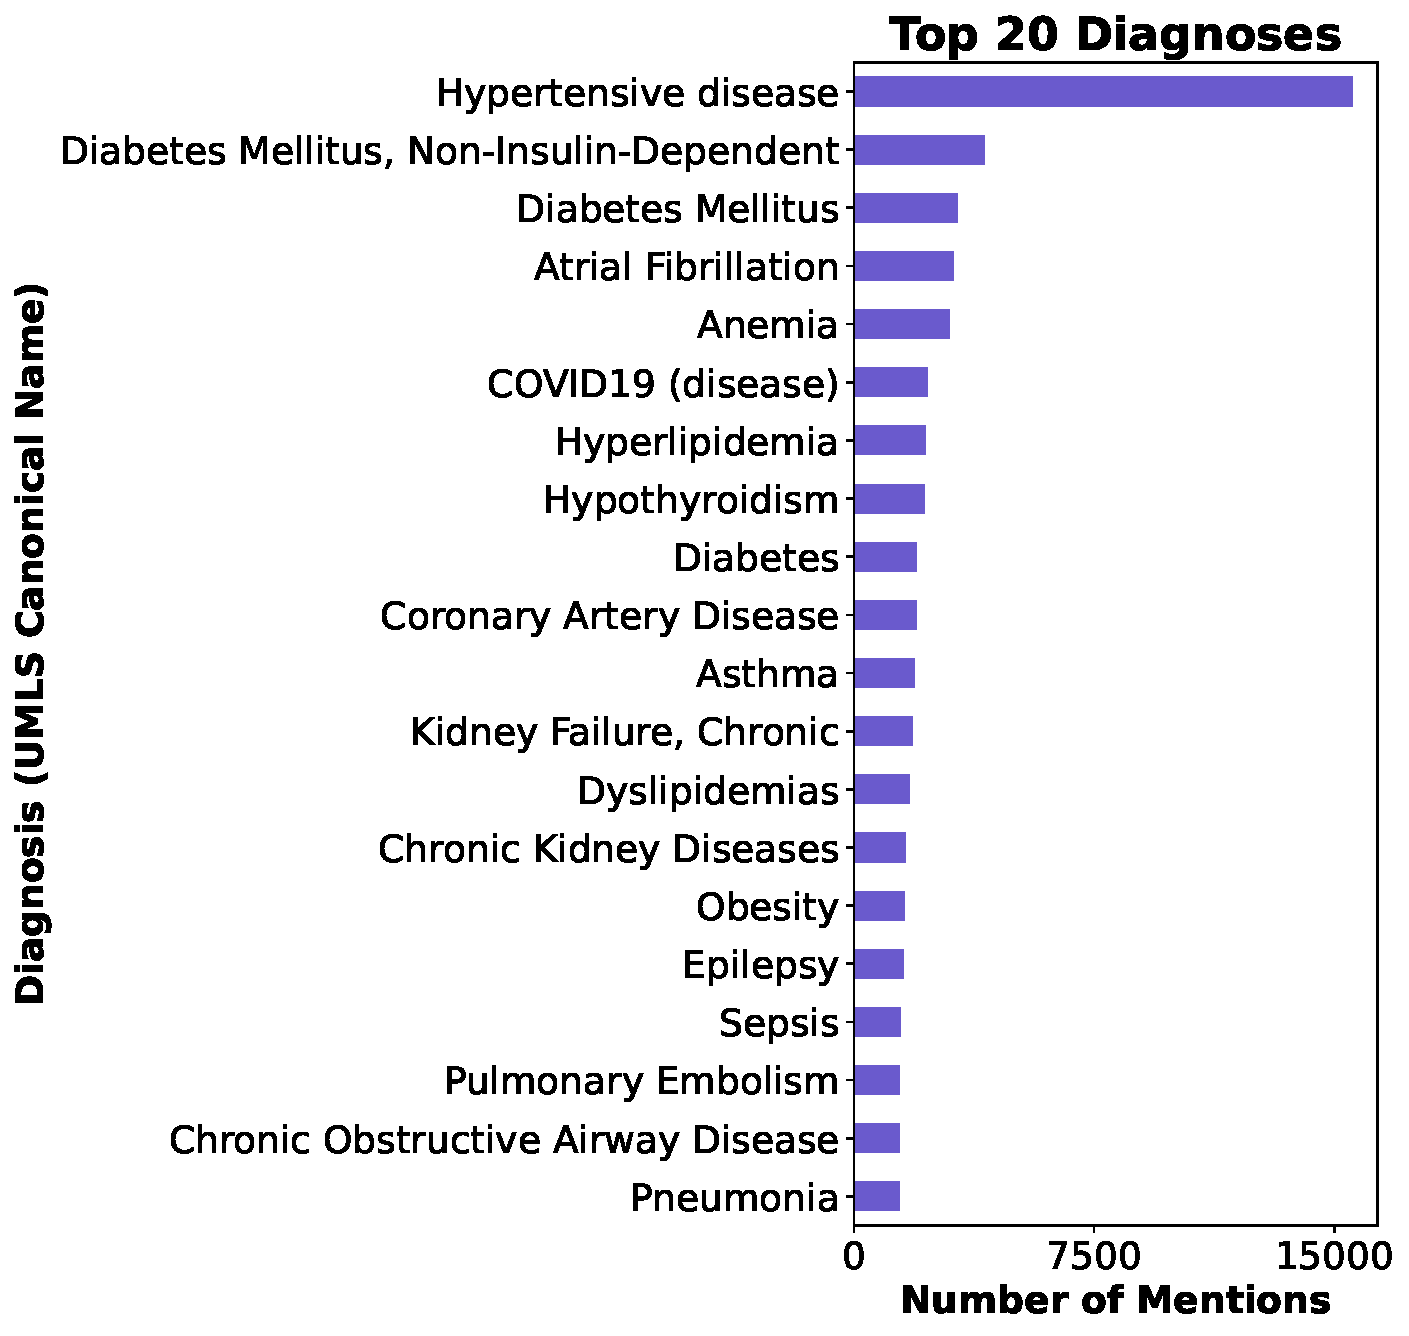
\includegraphics[width=0.99\linewidth]{Chapters/chapter-05/images/Scientific_data/Plots_tables/top_diagnoses_umls_corrected_lexical_tiebreak_paper_ready.pdf}}
        
        \label{ch05:fig:top_diagnoses}
    \end{minipage}}
    \hfill
    \subfloat[{Diagnosis co-occurrence heatmap.}]{\begin{minipage}[t]{0.6\textwidth}
        \centering
        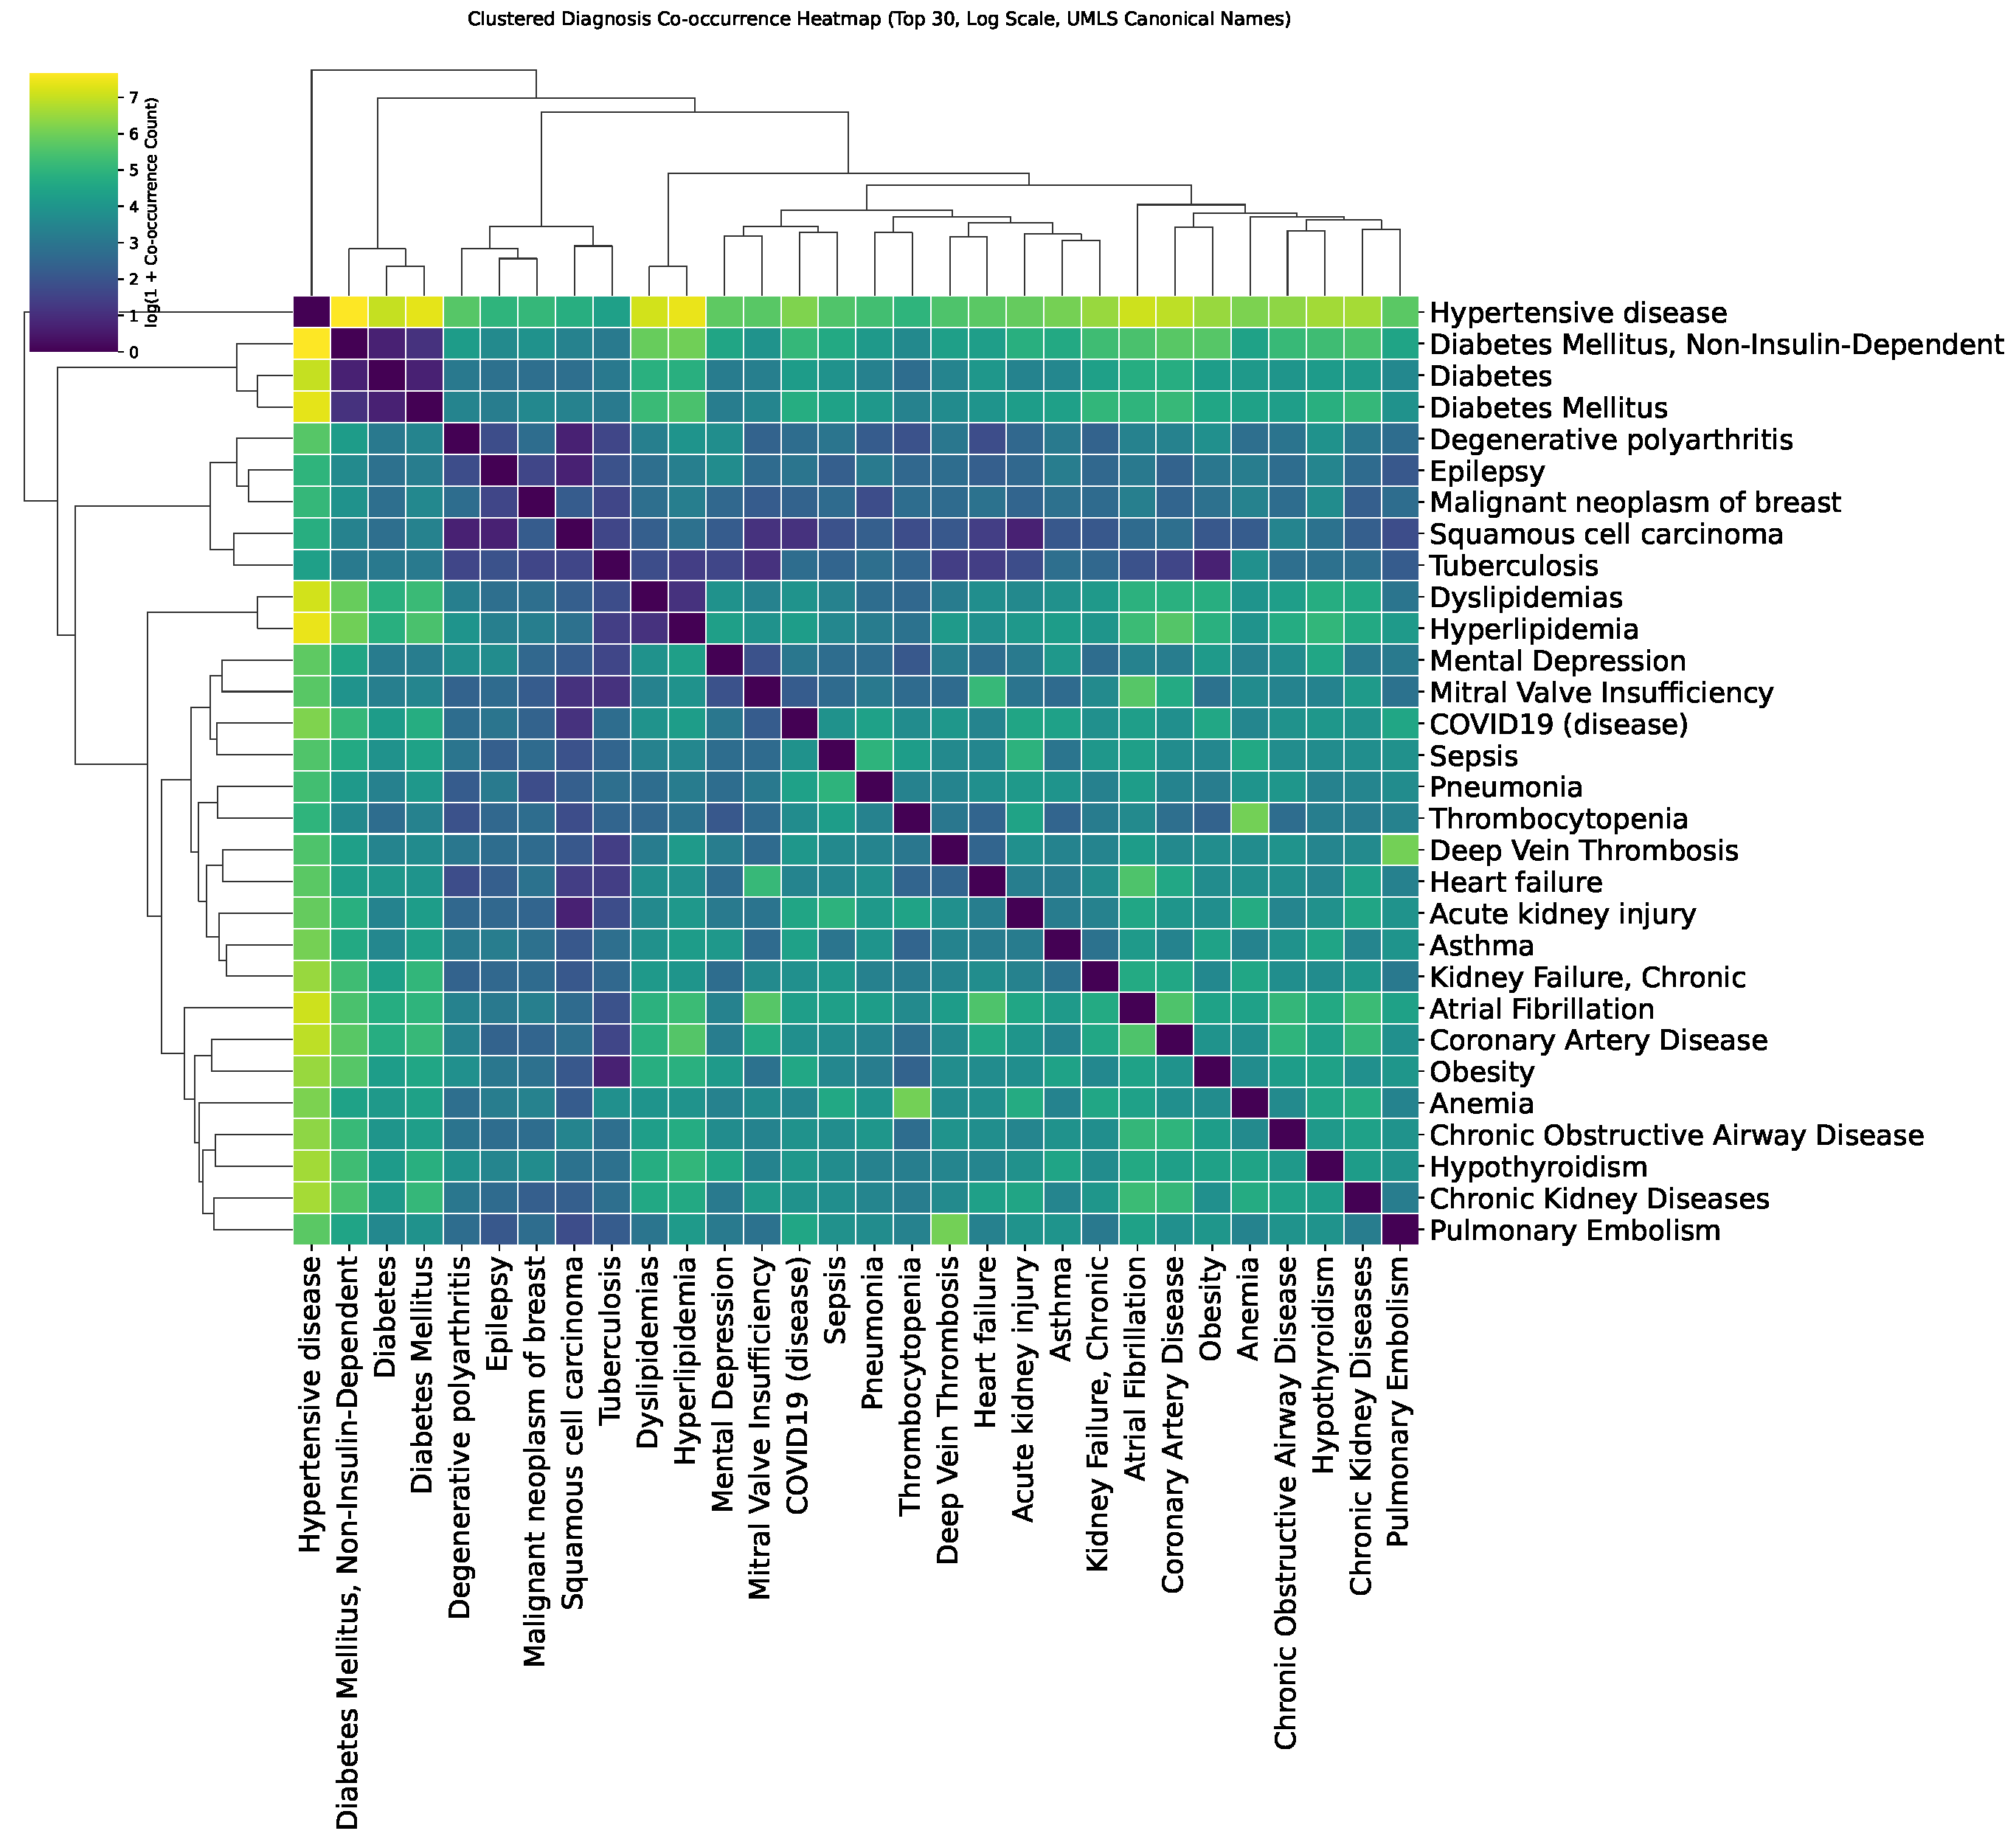
\includegraphics[width=0.99\linewidth]{Chapters/chapter-05/images/Scientific_data/Plots_tables/clustered_cooccurrence_heatmap_top30_corrected_lexical_tiebreak_canonical.pdf}
        
        \label{ch05:fig:diagnosis_cooccurrence}
    \end{minipage}}
    
    
    

\end{ChFiveFloatBody}
\caption{Frequency and co-occurrence patterns of UMLS-normalized diagnoses in PMOA-TTS. (a) The 20 most frequently mentioned diagnoses using canonical UMLS names. (b) Pairwise diagnosis co-occurrence (log-transformed counts) with hierarchical clustering, highlighting groups of frequently co-mentioned conditions.}\ChFiveFloatLabel{ch05:fig:diagnoses}
\end{figure}